165. \begin{figure}[ht!]
\center{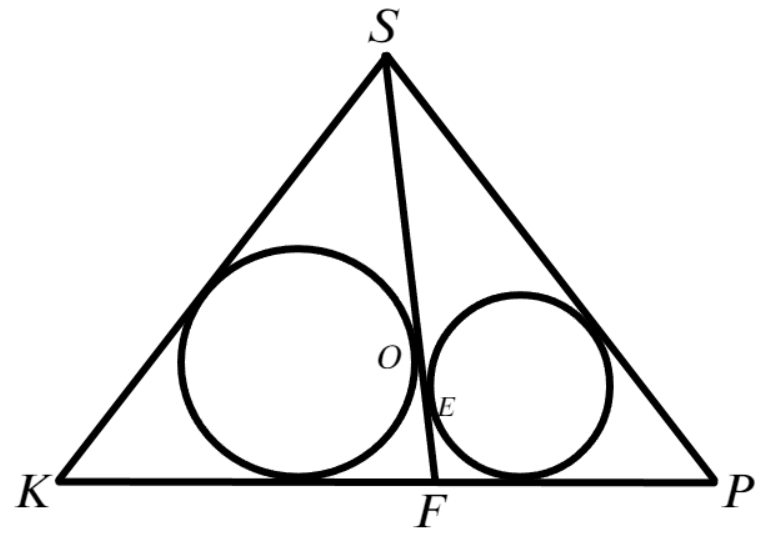
\includegraphics[scale=0.35]{g9-165.png}}
\end{figure}\\
По формуле для расстояния от вершины треугольника до точки касания имеем соотношения $FO=\cfrac{KF+SF-KS}{2},\ FE=\cfrac{PF+SF-SP}{2},$ тогда\\
$OE=FO-FE=\cfrac{KF+SF-KS}{2}-\cfrac{PF+SF-SP}{2}=\cfrac{KF-PF}{2}=\cfrac{3-1}{2}=1.$\\
